\documentclass{beamer}
\usepackage[utf8]{inputenc}
\usepackage[T1]{fontenc}
\usepackage[english]{babel}
\usepackage{graphicx}
\usepackage{times}
\usepackage{algorithm}
\usepackage{algpseudocode}
\usepackage{amsmath}
\usepackage{amssymb}
\usepackage{tikz}
\usetikzlibrary{calc,through,backgrounds,positioning,fit}
\usetikzlibrary{shapes,arrows,shadows}
%\usetheme{Rochester}
%\usetheme{Berkeley}
%\usetheme{Copenhagen}
\usetheme{Warsaw}
\title{6.5}
\author{A. Iksiński}
\institute{Wydział EAIiIB\\
	Katedra Informatyki Stosowanej}
\date{2015}
 \begin{document} 
 %-------------------------------------------------
\frame{\titlepage}
\begin{frame}
\frametitle{Zadanie 5.3}
\tikzstyle{place}=[shape=circle, draw, minimum height=10mm]
\tikzstyle{trig}=[shape=circle, draw, dashed, minimum height=10mm]
\tikzstyle{trans}=[shape=rectangle, draw, minimum height=6mm, minimum width=12mm] 
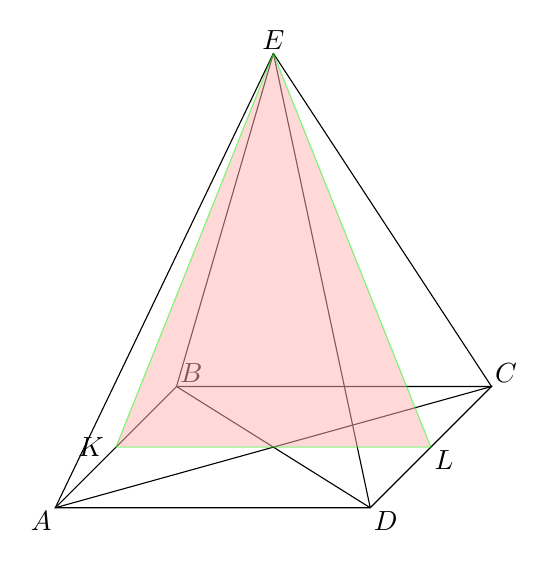
\begin{tikzpicture}[scale=1,inner sep=0.4mm]
\coordinate (A) at (0,0,4);
\coordinate (B) at (0,0,0);
\coordinate (C) at (4,0,0);
\coordinate (D) at (4,0,4);
\coordinate (E) at (2,5,2);
\coordinate (K) at (0,0,2);
\coordinate (L) at (4,0,2);	

\draw (A) node [below left] {$A$};
\draw (B) node [above right] {$B$};
\draw (C) node [above right] {$C$};
\draw (D) node [below right] {$D$};
\draw (E) node [above] {$E$};
\draw (A) -- (E);
\draw (B) -- (E);
\draw (C) -- (E);
\draw (D) -- (E);
\draw (A) -- (B) -- (C) -- (D) --cycle;\pause
\draw (B) -- (D);
\draw (A) -- (C);\pause
\draw (K) node [left=3pt] {$K$};
\draw (L) node [below right] {$L$}; 
\filldraw [draw=green,fill=red!30!white,opacity=0.5] (E) -- (K) -- (L) -- cycle;

\end{tikzpicture} 

\end{frame}
\begin{frame}[fragile]
\frametitle{Zadanie 5.5}
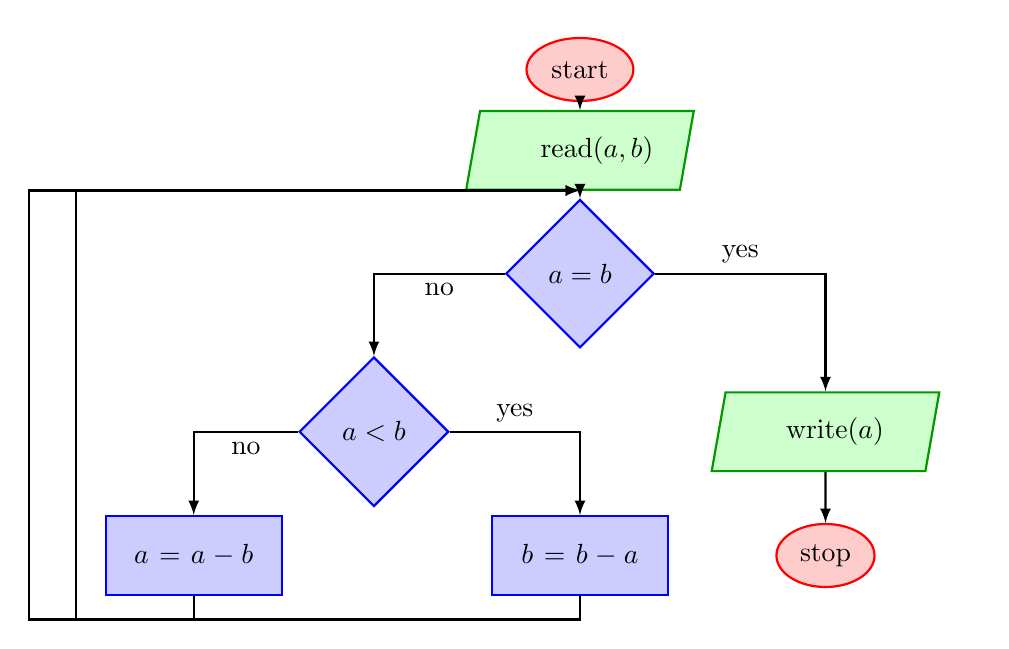
\begin{tikzpicture}[auto,
decision/.style = {diamond, draw=blue, thick, fill=blue!20, text width=1.5cm, 
	align=flush center, inner sep=1pt},
block/.style = {rectangle, draw=blue, thick, fill=blue!20, text width=2cm, 
	align=center, minimum height=1cm},
start/.style = {draw=red, thick, ellipse, fill=red!20, minimum height=8mm},
inout/.style = {draw=green!60!black, thick, fill=green!20, trapezium, trapezium left angle=80, align=center, trapezium right angle=-80, minimum height=10mm, text width=1cm, 
	inner sep=1pt},
line/.style ={draw, thick, -latex}]

\matrix[column sep=2mm,row sep=1mm]
{
	&& \node [start] (start) {start}; & \\
	&& \node [inout] (read) {read($a,b$)}; & \\
	&& \node [decision] (decide) {$a=b$}; & \\
	&\node [decision] (decide2) {$a<b$};  &&
	\node [inout] (write) {write($a$)}; \\
	\node [block] (block) {$a=a-b$}; &&
	\node [block] (block2) {$b=b-a$};
	& \node [start] (stop2) {stop}; &&\\
};
\begin{scope}[every path/.style=line]
\path (start) -- (read);
\path (read) -- (decide);
\path (decide) -| node [near start] {yes} (write);
\path (decide) -| node [near start] {no} (decide2);
\path (decide2) -| node [near start] {yes} (block2);
\path (decide2) -| node [near start] {no} (block);
\path (write) -- (stop2);
\path (block.south) -- ++(0,-.3) -- ++(-1.5,0) |- ($ (decide.north) + (0,0.1) $);
\path (block2.south) -- ++(0,-.3) -- ++(-7,0) |- ($ (decide.north) + (0,0.1) $);
\end{scope}


\end{tikzpicture}
\end{frame}
\end{document}

